\section{Contexto de uso}
\hspace{2.0cm}

Baseado no questionário aplicado foi contestado um insatisfação na forma atual
da prestação do serviço de "entrega e coleta de projetores", pelas partes
envolvidas. 

O questionário também aponta que a criação de um processo automatizado
satisfaria as partes envolvidas. 

\begin{center}
  \textbf{Link do Questionário professores}
  
  \href{https://goo.gl/forms/FzfGAn2JHJQKLoEq1}{questionário}

  \textbf{Relatório do Questionário professores}
  
  \href{https://goo.gl/S1c97v}{planilha}

  \textbf{Link do Questionário funcionário da secretária}

  \href{https://goo.gl/forms/FzfGAn2JHJQKLoEq1}{questionário}

\end{center}


O sistema visa solucionar esse gargalo com rapidez e confiança para ambas as
partes. 


\textbf{Possíveis Problemas}

Foi verificado também que os horários de picos para o uso do sistema são dos
horários CD - EF da Manhã e CD - EF da tarde, chegando as vezes ter falta de 
projetores. 


\subsection{Ambiente}

Observando o ambiente, local onde estão armazenado os projetores nota que e um
ambiente de fluxo alto e de pouco espaço para paradas e aglomeração de pessoas.
Fazendo pensar em uma solução que consuma o mínimo de tempo possível,
economizando tempo dos professores e evitando desgastes. 


\subsection{Proposta de Equipamento para implementação}

Um PC, Computador de mesa de baixa capacidade satisfaz aos requisitos, o sistema
seria web. 


\textbf{Pré-condições}


O sistema tem que estar entregado com o unifor-online. 


\textbf{Pós-condições}

Os usuários da secretária teria que serem cadastrados. 


\subsection{Descrição do contexto de uso antigo}


\textbf{Pegar o Projetor "Data Show"}


\begin{enumerate}
  
  \item O "usuário", interessa em pegar um projetor de imagem "Data show" dirigi-se ate a
  secretaria. 

  \item Nesse processo não ha verificação do case do projetor, da embalagem por
    nenhuma das partes. 

  \item Faz a solicitação de um projeto e preenche um formulário de papel com
    seu nome, numero do projeto, data do dia, nome do atendente e assina. 

\end{enumerate}

\textit{Diagrama do processo antigo de coleta dos projetores.}

  \begin{center}

    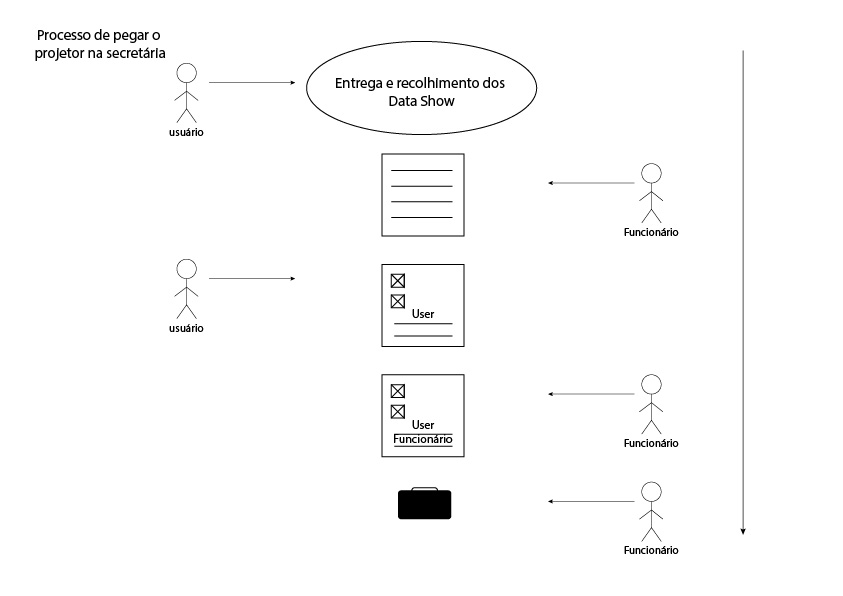
\includegraphics[scale=0.5]{imagens/fluxo1.jpg}\\

  \end{center}

\newpage


\textbf{Devolução do Projeto}

\begin{enumerate}
  
  \item O "usuário", de posse do projetor dirige para a secretária e faz a
    entrega a um atendente responsável. 

  \item É feita a verificação por parte do atendente, verificação do conteúdo do
    case. 

  \item É assinado o protocolo de entrega. 

\end{enumerate}


\textit{Diagrama do processo antigo de entrega dos projetores.}

  \begin{center}
    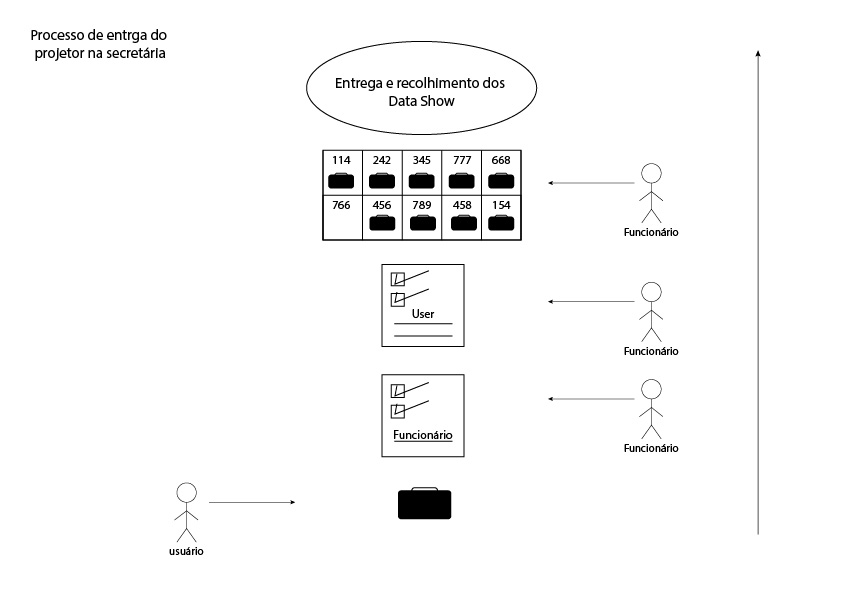
\includegraphics[scale=0.5]{imagens/fluxo3.jpg}\\
  \end{center}
  

\newpage

\subsection{Solução proposta do contexto de uso}

\textbf{Pedido do Projetor}

\begin{enumerate}

  \item O "usuário" dirige-se ate a secretária onde la tem um terminal de auto
    atendimento um PC onde ele entra no sistema com seu login e senha.

    \textit{Login}: Sua matricula e \textit{Senha:} Senha definida por ele no
    ato da criação de sua matricula.

  \item O sistema responde com uma tela de boa vindas e mostra os projetores
    disponíveis. 

  \item Após sua escolha e confirmação um usuário da secretária faz uma
    conferida no equipamento e adiciona se houver a necessidade de algum
    suplemento, digita seu pass e confirma a entrega do projetor.


\end{enumerate}


\begin{center}

  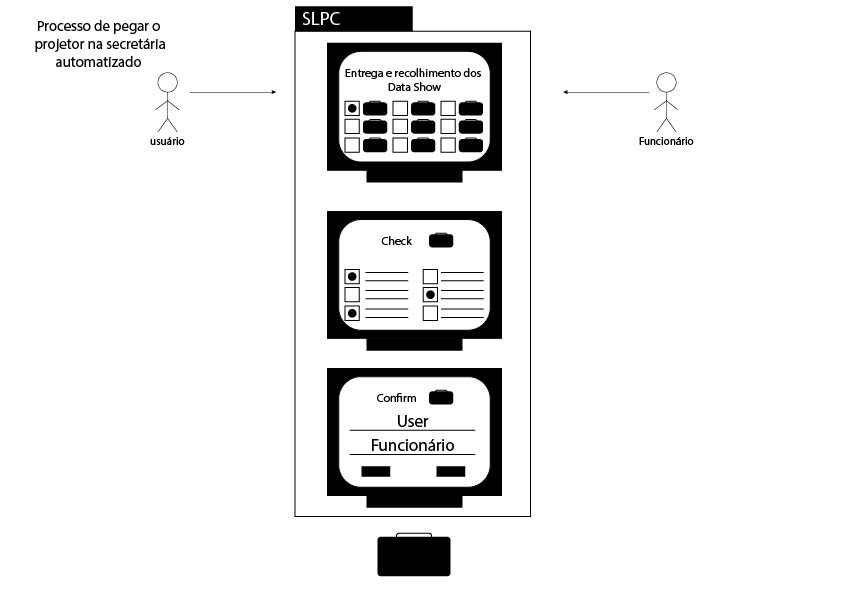
\includegraphics[scale=0.5]{imagens/fluxo2.jpg}\\

\end{center}

\subsection{Personas}


\begin{center}

  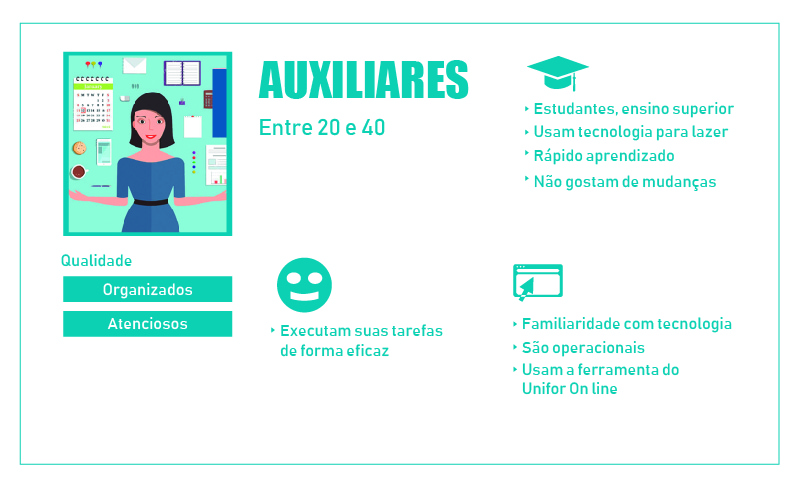
\includegraphics[scale=0.5]{imagens/persona.jpg}\\

  \textbf{Link da persona para melhor visualização}

  \href{https://goo.gl/Fv4L6r}{persona 1}

\end{center}

\begin{center}

  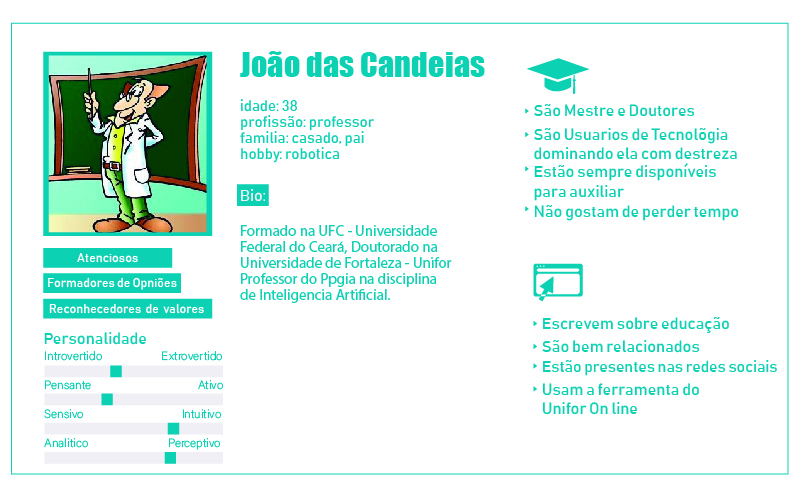
\includegraphics[scale=0.5]{imagens/persona2.jpg}\\

  \textbf{Link da persona para melhor visualização}

  \href{https://goo.gl/rTJupp}{persona 2}

\end{center}
